% Set up the document
%\documentclass[a4paper, 12pt, oneside]{bThesis} % My own class, based on the report class
%\documentclass[a5paper, 10pt]{bThesis} % Looks more like a book
%\documentclass[b5paper]{bThesis} % Looks more like a book
%\documentclass{bThesis} % Plain
\documentclass[oneside]{bThesis} % Plain
%\documentclass[a5paper,DIV=12,BCOR=9mm,headsepline,headings=small,cleardoubleempty,10pt]{bThesis} % Settings from Open Advise

% Info
\author{J\'on Bergmann Maronsson}
\title{\pending}

% Paths
\graphicspath{{figures/}}

% Start the document
\begin{document}

% The preamble stuff
% Titlepage
\begin{titlepage}
%\vspace{2cm}
%\noindent{\bf University of Iceland \\ Faculty of Natural Sciences \\ Department of Chemistry} \\ 
%\noindent \HRule \vspace{10mm}

%\begin{center}
%{\LARGE \bf Theoretical Calculations of }\\
%\vspace{3mm}
%{\LARGE \bf Electrochemical Systems }\\
%\vspace{8mm}
%\normalsize{by}\\
%\vspace{5mm}
%\large{ \bf J\'on Bergmann Maronsson}\\ \vspace{27mm}
%\includegraphics[width=45mm]{hi} \\ \vspace{27mm}
%\normalsize{ Thesis for the degree of  \\ Magister Scientiarum in Chemistry \\ October 2008}
%\end{center}
%
%\HRule
%
%\noindent \textbf{Thesis Advisor: Professor Hannes J\'onsson}\\
%\noindent \textbf{Co-Advisor: Associate Professor Yoshitada Morikawa }\\
%\noindent \textbf{External Examiner: Professor Vi\dh{}ar Gu\dh{}mundsson }

\maketitle

\includegraphics[width=1.0\linewidth]{paths}

\end{titlepage}


% Flyleaf
%\begin{titlepage}
% \hspace{10cm}
%\end{titlepage}

% Set the page count for the preamble
\pagestyle{plain}
\pagenumbering{roman}
\setcounter{page}{2}

% Include the preamble
\section*{Preface}
\addcontentsline{toc}{chapter}{Preface}

This thesis is submitted in candidacy for the Ph.D. degree from the Technical University of Denmark (DTU).
The work has been carried out over between November 2008 and February 2012 at the Ris\o{} DTU campus, formerly the Ris\o{} National Laboratory for Sustainable Energy, DTU; the Center for Atomic-scale Materias Design (CAMd) and with external stays at the University of Iceland.
The project was supervised by Tejs Vegge from the Technical University of Denmark and co-supervised by Hannes J\'onsson from the University of Iceland.
The project's funding was provided by \expand

\vspace{10mm}
\begin{flushright}
Kgs. Lyngby, February 29th 2012,\\

\vspace{15mm}

\rule{50mm}{0.1pt}\\
\textit{J\'on Bergmann Maronsson}
\end{flushright}

\newpage
\chapter*{Abstract}
\addcontentsline{toc}{chapter}{Abstract}

Reaction rates in theoretical chemistry was the main focus of this thesis.
Applying current methods to aid analysis of experimental data in complex borohydrides and improving these commonly used methods.

Complex borohydrides are materials of high hydrogen storage capacity and too high thermodynamic stability.
Understanding the high stability is of great importance to the development of suitable materials for hydrogen storage.
In an effort to gain insight into the structural transitions of two such materials, \ce{Ca(BH4)2} and \ce{Mg(BH4)2}, low temperature rotational dynamics experiments were performed.
The work presented in here revolved around assisting in the data analysis by performing density functional theory calculations on the possible dynamical events.
For the \ce{Mg(BH4)2}, only rotational dynamics were detected and they were in good agreement with the experimental values, showing that $C_2$-type rotations happen at lower temperatures than $C_3$-type rotations and that approximately $15\%$ of the \ce{BH4} units activate at a lower temperature than the rest.
For the \ce{Ca(BH4)2}, in addition to the rotational dynamics, longer range diffusion was detected.
Most likely this was due to \ce{H2}-interstitial defects.
The rotational dynamics were more prominent in the data and good agreement with the experiments was reached, showing that $C_3$-type rotations activate at lower temperatures than $C_2$-type rotations.

A method for finding the ridge between first order saddle points on a multidimensional surface was developed.
For atomic scale systems, such points on the energy surface correspond to atomic rearrangement mechanisms.
Information about the ridge can be used to test the validity of the harmonic approximation to transition state theory for reaction rates,
in particular to verify that second order saddle points - maxima along the ridge - are high enough compared to the first order saddle points.
Furthermore, corrections to the harmonic approximation can be estimated by direct evaluation of the configuration integral along the ridge.
New minima along the ridge can also be identified during the path optimisation,
thereby revealing additional transition mechanisms.
The method is based on modifying the gradient of a set of points along a path connecting the saddle points to iteratively converge to the ridge.
%The method is based on optimising a string of discretisation points along a path between the saddle points and using an iterative optimisation which requires only the force acting on the atoms.
At each iteration during the optimisation, the gradient is inverted along an unstable eigenmode perpendicular to the path, effectively mapping the ridge to a minimum energy path.
The method was applied to Al adatom diffusion on the Al(100) surface to find the ridge between 2-, 3- and 4-atom concerted displacement
and hop mechanisms for diffusion.

\newpage
% Rename the Icelandic abstract
%\renewcommand{\abstractname}{\'Agrip}
%\begin{abstract}
%\TH{}etta er frekar magna\dh{}.
 
%\end{abstract}
% Restore the abstract to English

%\begin{center}
%\section*{}
%\vspace{20mm}
\section*{Resum\'e}
\addcontentsline{toc}{chapter}{Resum\'e}

%\selectlanguage{danish}

Forståelse af reaktionshastigheder er en essentiel del af moderne forskning på atomar skala.
I denne afhandling beskrives anvendelsen af veletablerede metoder til beskrivelse af vigtige hydrogenlagrings-systemer. Herefter videreudvikles metoderne for at kunne opnå en bedre beskrivelse af reaktionsvejsomgivelserne, for herigennem at bestemme reaktionshastigheden med større nøjagtighed.

Komplekse borohydrider er materialer med en høj hydrogenlagrings-kapacitet og er yderligere meget termodynamisk stabile (for stabile til hydrogen lagring).
For at få bedre indsigt i de strukturelle overgange i to sådanne materialer, \ce{Ca(BH4)2} og \ce{Mg(BH4)2}, blev der udført lav-temperatur rotationsdynamik eksperimenter.
%(I am actually not sure what you mean excactly when talking about structural transitions, but I think this translation should suit most of it :-) furthermore I am not sure whether "rotationsdynamik" is the correct word to use - I do not know much (anything) about it.. so you should probably ask an expert :-) )
Arbejdet der præsenteres her omhandler assistance i forbindelse med dataanalyse, ved hjælp af tæthedsfunktionalteori-beregninger, på de mulige dynamiske hændelser.
For \ce{Mg(BH4)2}, var der god overensstemmelse med eksperimenter. $C_2$-type rotationer observeres ved lavere temperaturer end $C_3$-type rotationer og cirka $15\%$ af \ce{BH4}-enhederne aktiveres ved lavere temperaturer end resten.
For \ce{Ca(BH4)2} observeredes, udover rotationsdynamikken, en uidentificeret hændelse, som ifølge beregningerne sandsynligvis skyldes \ce{H2}-interstitielle defekter.
I god overensstemmelse med eksperimenter, aktiveres $C_3$-type rotationer ved lavere temperaturer end $C_2$-type rotationer.

For at undersøge reaktionsvejes omgivelser, blev der udviklet en metode til at finde højderyggen mellem førsteordens saddelpunkter på en multidimensional overflade.
Information om højderyggen kan bruges til at verificere den harmoniske approksimation brugt i forbindelse med transition-state-teorien anvendt til bestemmelse af reaktionshastigheder, specielt i forbindelse med verificeringen af at andenordens saddelpunkter, maksima langs højderyggen, er beliggende højere sammenlignet med førsteordens saddelpunkter.
%(I am not sure whether to use "ryg" or "højderyg" - the last one is used in geology and for describing mountains, whereas the first also simple means back (human's). Is multidimensional surface an OK word, it is only a surface if in 2d?. I do not think we have a Danish word for tst.)
Yderligere kan korrektioner til den harmoniske approksimation estimeres ved direkte evaluering af det konfigurative integerale langs højderyggen. (I am not sure about "konfigurative" have never heard about it..)
Nye minima langs højderyggen kan også identificeres sideløbende med reaktionsvejs-optimeringen, og derigennem kan yderligere transitions-mekanismer afsløres.
Metoden er baseret på modifikation af gradienten, for et sæt af punkter langs reaktionsvejen der forbinder saddelpunkterne, så den iterativt konvergerer mod højderyggen.
Ved hver iteration under optimeringen, inverteres gradienten langs en ustabil egentilstand vinkelret på reaktionsvejen. Dette afbilder effektivt højderyggen mod en minimum reaktionsvej, som kan findes med flere forskellige kendte teknikker.
Metoden blev anvendt til at studere Al adatom diffusion på Al(100) overfladen, for at finde højderyggen mellem en samlet bevægelse af 2, 3 eller 4 atomer, samt hoppe-mekanismer i forbindelse med diffusion.
Der var signifikante korrektioner for samlet bevægelse af 3 og 4 atomer. 
%(I am not sure if adatom is OK in Danish...)
Højderyg-metoden er en enkel metode som kan anvendes til at verificere reaktionshastigheder, men har potentialet for at bestemme mere nøjagtige hastigheder i sig selv, ved at repræsentere transition-state med højderyggen.



%\selectlanguage{english}

%\newpage 
%\chapter*{Acknowledgements}
\addcontentsline{toc}{chapter}{Acknowledgements}

\placeholder
%\begin{itemize}
% \item Professor Hannes J\'onsson, at the University of Iceland, for his guidance and inspiration.
% \item Associate Professor Yoshitada Morikawa, at the University of Osaka, for his guidance and kind manner while I was in a strange culture.
% \item Egill Sk\'ulason for collaboration, discussions and proof-reading.
% \item The members of the J\'onsson research group, at the University of Iceland, for enlightening discussions and support:
% \begin{itemize}
%  \item Sigr\'i\dh{}ur Gu\dh{}mundsd\'ottir, also for proof-reading
%  \item J\'on Steinar Gar\dh{}arsson M\'yrdal
%  \item Andreas Pedersen
%  \item Jean-Claude Berthet, Ph.D.
%  \item Peter Kl\"upfel, Ph.D.
% \end{itemize}
% \item The members of the J\'onsson research group, at the University of Iceland, for help with compilation issues, discussions and proof-reading:
% \begin{itemize}
%  \item Andri Arnaldsson, Ph.D.
%  \item Finnbogi \'Oskarsson
% \end{itemize}
% \item The members of the Yoshida research group, at the University of Osaka, for discussions, help and kind acceptance in a strange culture:
% \begin{itemize}
%  \item Susumu Yanagisawa, Ph.D.
%  \item Ikutaro Hamada, Ph.D.
%  \item Kunihiko Yamauchi, Ph.D.
% \end{itemize}
%% \item The best curry place in existence, Senba Curry, at the train station at Kita-Senri in Osaka, Japan.
% \item Friends and family for putting up with my studies for such a long time.
% \item Computer facilites: Bj\'olfur, J\"otunn and Itanium
% \item Funding:
% \begin{itemize}
%  \item Japanese Government (MONBUKAGAKUSHO:MEXT) Scholarship
%  \item Science Institute of the University of Iceland
% \end{itemize}
%\end{itemize}


% Tables of contents
\tableofcontents
%\listoffigures
%\listoftables

% Abbreviations
%\newpage
%\section{List of Abbreviations}

\begin{tabular}{rl}
TST & Transition State Theory \\
HTST & Harmonic Transition State Theory \\
SP & Saddle Point \\
\sap{1} & First Order Saddle Point \\
\sap{2} & Second Order Saddle Point \\
\sap{N} & $N$th Order Saddle Point \\
DFT & Density Functional Theory \\
QENS & Quasi-Elastic Neutron Scattering \\
BOA & Born-Oppenheimer approximation \\
\end{tabular}

%\newpage

% Reset the page count for the main content
\newpage
\pagestyle{plain}
\pagenumbering{arabic}
\setcounter{page}{1}


% Include the chapters
\part{Introduction}
\label{part:introduction}
\chapter{Introduction}
\label{chap:introduction}

%\bit
%\item Energy storage, conversion and mobility (Hydrogen as an example)
%\item The importance of assessing reaction rates (Kinetics is a very important aspect for the above)
%\item General problems with getting reaction rates
%\item Annoying landscapes
%\item Beyond harmonicity
%\item The methods presented here are not exclusive to atomistic simulations
%\eit

Stationary points of functions are interesting for a number of reasons \expand




\subusbsection{Old Methods Introduction}
The focus of this thesis is the application of theoretical methods to calculational reaction chemistry.
The underlying methods that allow this are numerous and their discovery span ages in time, from Newton's equations of motion~\cite{newton-latin} up to modern day methods for solving Sch\"odinger's equation~\cite{schrodinger-equation-1926} for quantum systems\cite{hohenberg-kohn-1964, gpaw-review-2010}, from the discovery of calculus\citemiss\footnote{see Leibnitz: \url{http://books.google.dk/books?id=UdGBy8iLpocC&pg=PA46&redir_esc=y\#v=onepage&q&f=false}} and vector math~\citemiss to modern methods for solving eigenvalue problems\citemiss.
%This chapter will give a brief look at the main methods employed with special emphasis on those that constitute the basis of the novel method presented in \fref{chap:erm}.

Simulations of atomic systems are an integral part of modern atomic scale research, whether it be to investigate specific electronic structure properties\citemiss, performing atomic dynamics\citemiss or investigating macroscopic properties\citemiss.
Simulations are commonly employed in the analysis of interesting material properties (see for example catalytic properties\citemiss), the screening of candidate materials --- to eliminate the need to synthesize as many unsuccesful materials --- for various processes (see for example hydrogen storage\citemiss) and further collaboration and comparison with experiments (see for example \citemiss).

Reaction chemistry happens on a timescale of microseconds which is, essentially, eternity when seen from the vantage point of the fast moving vibrations, which happen on a timescale of femtoseconds.
Briding this gap is an important research subject which remains open, despite noble efforts that have moved the field a long way\citemiss.

%Dating back to well before modern large scale computer clusters, synamical studies were even performed using tools no more complicated than balls, sticks, pens and paper~\cite{old-simulations-bernal-1962} ATH: Vegetable Staticks (Stephen Hales, 1727)


%\tblue{The order of the topics for discussion in this chapter is still a bit off.
%Born-Oppenheimer is needed before TST but it should be introduced at the same (similar) time as the Schr\"odinger equation which in turn should accompany the DFT section (close to which the potential function section should lie).}
%\bit
%\item Perhaps use the Newton/Schr\"odinger figure I made a bit back (modified if needed)
%\item General on atomistic simulations (seguing to potential functions and DFT)
%\item Why statistical methods
%\item Why path techniques (introduction to be expanded on in the TST section)
%\item It is now "possible" to do long timescale MD simlations but statistical methods are still more suited to find "all" the processes (chat with Elvar on MD)
%\item (Why these methods but not some other?)
%\item Methods that or of particular interest get better coverage.
%
%\item Would be nice to have a figure of each of the main guys for each methodology
%\bit
%\item Born, Oppenheimer
%\item Hesse
%\item Arrhenius, Kramer
%\item Hannes, Graeme
%\item Hohnberg, Kohn
%\eit
%\eit


%\section{Notation}
%\bit
%\item Nuclei positions: $\vR$
%\item Electron positions: $\vr$
%\item R-basis for formulas
%\item The PES: $E(\vR)$
%\eit

\section{Chapter Outline}
\label{sec:chapters}

The papers will not be retold, but rather summarised and expanded on, in their respective chapters.

\subsubsection{\Fref{chap:methods}}
The methods and concepts that are important to the work presented in the thesis are discussed.
This chapter is not intended as an exhaustive resource for the methods in question but more as an introduction, sufficient to understand the thesis.
For more in-detail discussion of individual methods, refer to their respective citations.

\subsubsection{\Fref{chap:borohydrides}}
Metal Borohydrides \expand

\subsubsection{\Fref{chap:erm}}
Beyond Harmonicity \expand

\subsubsection{\Fref{chap:al}}
Self-Diffusion of Aluminium \expand

\subsubsection{\Fref{chap:perovskites}}
Coupled Hydrogen Defects \expand



\part{Theoretical Methods}
\label{part:theory}
\chapter{Methods}
\label{ch:methods}
\section{Introduction}
\label{sec:methods-introduction}

% ------------------------------------------------------------------
\bit
\item Perhaps use the Newton/Schr\"odinger figure I made a bit back (modified if needed)
\item General on atomistic simulations (seguing to potential functions and DFT)
\item Why statistical methods
\item Why path techniques (introduction to be expanded on in the TST section)
\item It is now "possible" to do long timescale MD simlations but statistical methods are still more suited to find "all" the processes (chat with Elvar on MD)
\item (Why these methods but not some other?)

\item Would be nice to have a figure of each of the main guys for each methodology
\bit
\item Born, Oppenheimer
\item Hesse
\item Arrhenius, Kramer
\item Hannes, Graeme
\item Hohnberg, Kohn
\eit
\eit

The order of the topics for discussion in this chapter is still a bit off.
Born-Oppenheimer is needed before TST but it should be introduced at the same (similar) time as the Schr\"odinger equation which in turn should accompany the DFT section (close to which the potential function section should lie).

\placeholder

\section{Important Concepts}
\label{sec:important-concepts}

This secion shortly introduces a few concepts that are important to the work being presented.

\incomplete
% ------------------------------------------------------------------
\subsection{The Born-Oppenheimer Approximation}
\label{sec:born-oppenheimer}

In order to simplify calculation of large atomic systems, the difference in weight of the electrons and the nuclei is exploited by performing tha calculations in two steps.
First the electronic wavefunction is determined while the nuclei are kept fixed followed by a calculation for the motion of the nuclei while the electronic wavefunction is kept fixed.

\bit
\item Introduce PES
\eit

\incomplete

% ------------------------------------------------------------------
\subsection{Eigenmodes / Eigenvalues}
\label{sec:eigenmodes}

\placeholder

% ------------------------------------------------------------------
\subsection{Reduced Vector-space}
\label{sec:reduced-space}

\placeholder

% ------------------------------------------------------------------
\subsection{The Hessian Matrix}
\label{sec:hessian}

For a real function $f$ of $n$ variables, $\vect{x} = (x_1, x_2, \ldots, x_n)$,
there exists an $n\times n$ matrix, $H$, which contains all the second partial derivatives, if they exist,
\beq{hessian-matrix}
H =
\begin{bmatrix}
\vspace{0.5em} % To create a bit of space AFTER the first line.
\frac{\partial^2f}{\partial x_1^2} &
\frac{\partial^2f}{\partial x_1 \partial x_2} &
\cdots &
\frac{\partial^2f}{\partial x_1 \partial x_n} \\

\frac{\partial^2f}{\partial x_2 \partial x_1} &
\frac{\partial^2f}{\partial x_2^2} & 
\cdots &
\frac{\partial^2f}{\partial x_2 \partial x_n} \\

\vdots & \vdots & \ddots & \vdots \\

\frac{\partial^2f}{\partial x_n \partial x_1} &
\frac{\partial^2f}{\partial x_n \partial x_2} &
\cdots &
\frac{\partial^2f}{\partial x_n^2} &
\end{bmatrix}
\eeq
The second derivative of a function represents, in particular, information about its local curvature, or how rapidly the first derivative changes.
$H$ is named after the German mathematician Ludwig Otto Hesse and is commonly referred to as the Hessian matrix, or Hessian for short. \tred{[original ref]}

In the context of atomic simulations $n$ is generally 3 times the number of atoms in the system, as each one has 3 independant degrees of freedom.
The function in question is often the potential energy of the system, whose negative gradient is commonly referred to as the force.
In most modern software packages both the potential energy and force are readily available while the second derivatives are, generally, not available without explicit and, often, costly calculations.

\recent

% ------------------------------------------------------------------
\subsection{Saddle Points}
\label{sec:sps}

Saddle points are stationary points, i.e. with zero gradient, on multidimensional function, $f(\vR)$, that are neither maxima nor minima.

The most common image of a saddle (point) is the function $f(x, y) = x^2 - y^2$ which near $(x,y) = (0,0)$ resembles a saddle, used when riding horses (se figure...), curving upwards in one direction and downwards in the other.
\figmiss{Comparison of a saddle points environment and a saddle used on a horse.}
This most common image of a saddle point lacks a few elements to be to tell their whole story.

On functions of higher dimensionality than $2$, different orders of saddle points are possible.
The order of the saddle point is decided by the amount of directions that are at a maximum, rather than a minimum.
As such, figure ... show a first order saddle point on a two dimensional function.

\bit
\item What about 1D saddles (e.g. $f(x = 0) = x^3$)
\item What about similar constructs in more dimensions (e.g. like the above in one direction but a maximum in the other)
\eit

\recent

\incomplete

% ------------------------------------------------------------------
\subsection{Steepest Decent Paths}
\label{sec:sdps}


\placeholder

Two sorts of SDPs are of particular interest for the work carried out here and are discussed below.

% ------------------------------------------------------------------
\subsubsection{Minimum Energy Paths}
\label{sec:meps}

\placeholder

% ------------------------------------------------------------------
\subsubsection{Ridges}
\label{sec:ridges}

Special steepest decent paths, which do not end at minima but saddle points.

\placeholder



\section{First Order Saddle Point Methods}
\label{sec:sps}

Finding saddle points is a non-trivial task in multiple dimensions, when only local information is available and computational resources are limited, such that calculation of the Hessian matrix is infeasible.

\incomplete

% ------------------------------------------------------------------
\subsection{Nudged Elastic Band}
\label{sec:neb}

Finding Steepest Decent Paths (SDPs) from a given point is simple by following the gradient with a small step size.
On the other hand, finding specific SDPs that end at minima is not.
The goal here is to find two SDPs each leading from the same \sap1 to different minima without any further information than the minima.


\incomplete

% ------------------------------------------------------------------
\subsection{Dimer}
\label{sec:dimer}

The Dimer method was inspired by Voter\cite{voter-hyperdynamics-1997}

Given only an initial point, $\vR$, on a multidimensional function, $V(\vR)$, the goal is to, iteratively, locate a nearby \sap1, using no direct calculation of the Hessian, i.e. using only functional values and the gradient, $\nabla V(\vR)$.
Indirect information about the Hessian is, however, used in the form of an estimate of the eigenmode corresponding to its lowest eigenvalue (minimum mode).
Using the minimum mode, $\uvn$, it is possible to locally transform \sap1s to minima and using conventional techniques to move up-hill and locate the \sap1.

The dimer method can be split into three independent phases.
\ben{dimer-phases}
\item Estimating the minimum mode.
\item Transforming the gradient to make \sap1 seem as minima.
\item Translating the point according to the transformed gradient.
\een

\subsubsection{Minimum Mode Estimation}
Estimating the second derivative of $V$ along a given unit vector, $\uvs$, at point $\vR$ can be done numerically, using finite differences.
For the occasion, a pair of points (the dimer), $[\vR_\text{A}, \vR_\text{B}]$, are chosen, close to current point $\vR_0$, such that
\beq{dimer-separation}
\vR_\text{A} = \vR_0 + \Dsep \uvs \quad \text{and} \quad \vR_\text{B} = \vR_0  - \Dsep \uvs,
\eeq
where $\Dsep$ is a predefined constant to determine the length of the dimer and the separation in the finite difference estimate.
Using only the functional values
\beq{second-derivative-function}
C_\vs \equiv \frac{\partial^2 V}{\partial \uvs^2} \approx \frac{V_\text{A} + V_\text{B} - 2V_0}{\Dsep^2},
\eeq
where $V_\text{x} \equiv V(\vR_\text{x})$ and $C_\vs$ is the curvature or second derivative.
As gradient points away from each minimum, it is convenient to define a force, $\vF$ that points towards minima instead, for use in the iterative minima search,
\beq{gradient-force}
\vF_\text{x} \equiv - \nabla V(\vR_\text{x}).
\eeq
If the gradient is readily available, \fref{eq:second-derivative-function} can be rewritten to depend on it instead,
\beq{second-derviative-gradient}
C_\vs \approx \frac{(\vF_\text{B} - \vF_\text{A}) \cdot \uvs}{\Dsep}.
\eeq

Rotating $\uvs$ around $\vR_0$ until $C_\vs$ is minimized yields an estimate for, both, the lowest eigenvalue, $C_\text{min} = C_\vs$, of the Hessian and it corresponding eigenmode, the minimum mode, $\uvn$.


%The manner in which this rotation is performed is varied...

%% Need to introduce the gradient as a symbol first....
%Often $f(\vR_0)$ has either been evaluated or needs to be.
%This can be taken advantage of as this neccesary calculation can be used to extrapolate values for one of the end points.
%To illustrate this $f(\vR_0)$ and $f(\vR_\text{A})$ have already been calculated.
%The value at $\vR_\text{B}$ can then be extrapolated,
%\beq{dimer-extrapolate}
%f(\vR_\text{B}) = 2f(\vR_0) - f()
%\vR_\text{}
%\vR_\text{}
%\vR_\text{}
%\vR_\text{}
%\vR_\text{}
%\vR_\text{}
%\eeq

\incomplete

\subsubsection{Gradient Transformation}
Once a minimum mode estimate is available for the current point, $\vR_0$, it is possible to transform the gradient so that any \sap1 is transformed to a minimum.
\beq{dimer-transform}
\nabla{}f(\vR_0)
\eeq

\tblue{This latter step is not unique to the dimer algorithm... Lancoszs...}

\incomplete

\subsubsection{Iterative Translation}

\incomplete

\section{Quantum Calculations}
\label{sec:methods-QM}

With increased computing power and, in particular, advances in parallel algortims, it is now possible to calculate a range of physical properties for materials on the atomic level without the use of any experimental parameters.
Such \textit{ab initio} (from the beginning) methods ...
\expand

\subsection{The Electronic Structure Problem}
The Schr\"odinger equation is the quantum analoge of Newton's equations of motion and thus governs the motions of the quantum system in question as well as its observables.
\expand

The Born-Oppenheimer approximation (\fref{sec:born-oppenheimer}) allows the separation of the Hamiltonian to an electronic part and a nuclear part.
Thus, the positions of the nucleii, $\vR_I$ only enter the calculations as parameters.
A full quantum treatment will not be discussed here.
\expand

A non-relativistic system of $N$ electrons (and $N_I$ nuclei) is described by the time independant Schr\"odinger equation,
\beq{schrodinger-basic}
 \widehat{H}\Psi = E\Psi,
\eeq
where $\Psi \equiv \Psi(\vr_1, \vr_2, \ldots ,\vr_N)$ is the wave function, depending on the spatial coordinates, $\vr_i$, of each electron, $E$ is the electronic energy of the system and $\widehat{H}$ is the hamiltonian,
\beq{hamiltonian}
\widehat{H} = -\sum_i^N \frac{\nabla^2_i}{2} - \sum_i^N \sum_{j>i}^N \frac{1}{\left| \vr_i - \vr_j \right|} - \sum_i^N \sum_I^{N_I} \frac{1}{\left| \vr_i - \vR_I \right|} + V_\text{env},
\eeq
which consists of 4 terms.
First there is the kinetic energy of the electrons, then the electron-electron interaction, followed by the electron-nuclei interaction and finally any further environmental influence (e.g. an applied electric field) is represented by a single term.
The last two terms are often bundled into a single external term,
\beq{hamiltonian-external}
V_\text{ext} = \sum_i^N \sum_I^{N_I} \frac{1}{\left| \vr_i - \vR_I \right|} + V_\text{env}.
\eeq

Though it may look innocent, solving the Schr\"odinger equation, which is a second order partial derivative problem \tred{(is this correct?)}, is a daunting task and in most cases significant approximations must be made.
In particular, storing the wavefunction of a large system requires more data capacity than practical. \expand

\subsection{Density Functional Theory}
\label{sec:methods-dft}
One of the most popular and common teqchniques for solving the electronic structure problem is the Density Functional Theory (DFT) which can, from first principles (\textit{ab initio}), exactly (in theory) solve the Schr\"odinger equation.
However, in practice, approximations must be made for all but the most simple systems.
Nevertheless, DFT has produced many interesting and good results and is now a well established formalism that is continually being reviewed and improved.
Furthermore, the \textit{ab initio} nature of DFT makes it a great companion to experimental research, not only for comparison and prediction of interesting materials but also to assist and expand upon data analysis.

The success of DFT has yielded one of its founders, Walter Kohn, one half of the Nobel Prize in chemistry in 1998, for the development of the density functional theory~\cite{kohn1999} along with John Pople for his development of computational methods in quantum chemistry~\cite{pople1999}.

\subsubsection{The Hohenberg-Kohn Theorem}
The origin \tblue{(What about the Thomas-Fermi model)} of DFT lies in the Hohnberg-Kohn theorem, which reformulates the electronic structure problem to depend on the $3$ dimensional, ground state, electron density, $\rho(\vr)$, instead of the $3N$ dimensional wavefunction, $\Psi(\vr_1, \vr_2, \ldots, \vr_N)$.
According to the first Hohenberg-Kohn theorem~\cite{hohenberg-kohn-1964}, any external term, $V_\text{ext}$, in \fref{eq:hamiltonian} yields a different electron density from any non-identical, up to a constant, $V'_\text{ext}$.
In other words: there is a one-to-one correspondence between the wavefunction and the electron density of the ground state and all observables that depend on the wavefunction can, thus, be extracted from the ground state density.
Furthermore, the second Hohenberg-Kohn theorem~\cite{hohenberg-kohn-1964} adds a variational way to discover the true ground state density and thus ground state energy, $E_0$.

A re-formulation of the Schrodinger equation, shows the energy as a functional of the electron density, $E[\rho(\vr)] = \bra a |b | c \ket$\expand

\tred{Revised until here}

Once this has been established, it is simple to see that the total energy is a unique functional of the electron density, $\rho(\textbf{r})$, which is an observable while the wavefunction is not,
\begin{equation}
\label{eq:H-KenergyDensity}
 E[\rho] = \langle \Psi[\rho] | \widehat{H} | \Psi[\rho] \rangle.
\end{equation}
The Raleigh-Ritz variational principle is used to minimize the energy and find the ground state and density, %[missing ref]
\begin{equation}
 E_{0} = \min_{\rho(\mathbf{r})} \left(E[\rho(\mathbf{r})] \right).
\label{eq:H-Kvariational}
\end{equation}
This is the basis of DFT, developed by Hohenberg and Kohn \cite{hohenberg1964} in 1964.

\bit
\item The earliest mention of DFT type calculations were made by Thomas~\citemiss and Fermi~\citemiss.
\eit

\subsubsection{The Kohn-Sham Equations}
Currently there is no known way to perform the one-to-one mapping suggested by the H-K theorem. However in 1965 Kohn and Sham (K-S) published an indirect approach for calculating the energy functional $E[\rho]$ \cite{kohn1965}.
They showed that the interacting many-electron system can be mapped, approximately, onto a non-interacting system of single electron states, $\{\phi_i\}$, where each electron is subject to the effective potential $v_{eff}(\vect{r})$ due to all other particles. These one electron wavefunctions can be produced by solving the K-S equations,
\begin{equation}
\label{eq:K-Sequation}
 \left\{-\frac{1}{2} \nabla ^2 + v_\mathrm{eff}(\vect{r}) \right\} \phi_i(\vect{r}) = \epsilon_i \phi_i(\vect{r}).
\end{equation}
Since both the effective potential and the wavefunctions are unknown these equations must be solved self-consistently.
The electron density can then be produced using the square of the wavefunctions,
\begin{equation}
\label{eq:electronDensity}
 \rho(\vect{r}) = \sum_{i=1}^N \left| \phi_i(\vect{r}) \right|^2.
\end{equation}
The effective potential can be written as
\begin{equation}
\label{eq:effectivePotential}
 v_\mathrm{eff}(\vect{r}) = v(\vect{r}) + v_{H}(\vect{r}) + v_{XC}(\vect{r})
\end{equation}
where $v(\vect{r})$ is the sum of the potential due to the kinetic and ionic parts in equation \ref{eq:generalHamiltonian}%[Is this correct and do I need to include this reference]
, $v_{H}(\vect{r})$ is the Hartree potential,
\begin{equation}
\label{eq:hartreePotential}
 v_{H}(\vect{r}) = \int d^3r \frac{\rho(\vect{r'})}{\left| \vect{r} - \vect{r} \right|},
\end{equation}
and
\begin{equation}
\label{eq:XCpotential}
 v_{XC}(\vect{r}) = \frac{\delta E_{XC}[\rho]}{\delta \rho(\vect{r})}
\end{equation}
is the potential due to the exchange-correlation functional, $E_{XC}[\rho]$, which will be discussed in section \ref{sec:XCfunctional} 

\subsubsection{The Exchange-Correlation Functional}
\label{sec:XCfunctional}
The Kohn-Sham equations are in principle exact, however the exchange-correlation functional, $E_{XC}[\rho]$, is generally not known and has to be approximated. The accuracy of the approximation becomes a major issue in solving the Kohn-Sham equations.

The exchange-correlation functional is a local functional which describes the electron-electron interaction,
\begin{equation}
\label{eq:XCfunctional}
 E_{XC}[\rho] = \int d^3r\, \epsilon_{XC}(\rho, \vect{r})\rho(\vect{r})
\end{equation}
where $\epsilon_{XC}(\rho, \vect{r})$ is the exchange-correlation energy density.

The approximations used in our work are based on the so-called Generalized Gradient Approach (GGA). The GGA uses the the exchange-correlation energy of a homogeneous electron gas at point $\vect{r}$ like the Local Density Approximation (LDA) \cite{kohn1965} but also uses the gradient of the density to account for inhomogeneity. This, however, is not a good choice by itself so a reduced density gradient, $s(\vect{r})$, is used, as suggested by Langreth and Perdew \cite{langreth1977}. The exchange-correlation functional then becomes
\begin{equation}
  E_{XC}^{GGA}[\rho] = \int d^3r\, \epsilon_{XC}^{GGA}(\rho(\vect{r}), s(\vect{r}))\rho(\vect{r})
\end{equation}
with
\begin{equation}
\label{eq:GGAreducedDensityGradient}
 s(\vect{r}) = \frac{\left|\nabla \rho(\vect{r})\right|}{2\sqrt[3]{3\pi^2\rho(\vect{r})} \rho(\vect{r})}.
\end{equation}
%The calculations in chapter \ref{ch:japan} use GGA based on the PBE functional \cite{perdew1996} while the calculations in chapter \ref{ch:dacapo} use GGA based on the RPBE functional \cite{hammer1999}.

\subsection{Implementation of DFT}
\label{sec:methods-dft-implemetnation}

\subsubsection{The Plane Wave Basis Set}
In implementing DFT calculations, the Kohn-Sham wavefunctions are expanded in a particular basis set. In our work plane waves are used under periodic boundary conditions in accordance with Bloch's theorem,
\begin{equation}
\label{eq:blochsTherom}
 \psi_\vect{k}^{m}(\vect{r}) = \sum_\vect{G}c_{\vect{k} + \vect{G}}^m\, e^{i(\vect{k}+\vect{G})\cdot\vect{r}}
\end{equation}
where $\vect{G}$ are the reciprocal lattice vectors. %[what are $c_{\vect{k} + \vect{G}}^m$?]. 
For an exact solution, an infinite number of plane waves is needed. Fortunately the plane waves at the lower end of the kinetic energy range are the most important, so the number of plane waves can be reduced by defining a cutoff, $G_{cut}$, where the solution becomes good enough:
\begin{equation}
 \left( \frac{\hbar^2}{2m} \right) \left| \vect{k} + \vect{G}_{cut} \right|^2 \le E_\mathrm{cut}.
\end{equation}
This leads to one of the main advantages of plane waves. By increasing the cutoff the accuracy of the calculation can be systematically increased. 

A disadvantage of plane waves is their inefficiency to deal with high curvature regions, such as the atomic core. To overcome this pseudopotentials can be used. In the core, pseudopotentials are an average of the potential due to the core electrons and the nucleus felt by the valence electrons inside a given sphere but outside the sphere the pseudopotential becomes identical to the all-electron potential. The plane-wave cutoff can be lowered even further when using pseudopotentials while generally giving results of good accuracy, especially the so-called ultrasoft pseudopotential with non-local components \cite{vanderbilt1990}.


\part{Thesis Proper \pending Discussion?} 
\label{part:thesis}
\chapter{Metal Borohydrides}
\label{chap:borohydrides}
\textit{This chapter describes and expands the theoretical work performed for Papers \ref{pap:calcium} and \ref{pap:magnesium} while commenting on the interaction between theoretical and experimental work.}
\section{Introduction}
\label{sec:borohydrides-introduction}


Tejs' comments
\bit
\item Order/Disorder transitions
\item Difficult to get atomic level experimental data
\item Multiple phases
\item Structures are not fully known (but mostly)
\item Large superstructures
\eit

This chapter describes the theoretical work performed for Papers \ref{pap:calcium} and \ref{pap:magnesium} while commenting on the interaction between theoretical and experimental work.

The high hydrogen density, both volumetric and gravimetric, of metal borohydrides makes them interesting research topics as candidates for hydrogen storage.
However, they commonly exhibit poor reversability~\citemiss, slow ab- and de-sorbtion kinetics~\citemiss and too high thermodynamic stability~\citemiss.
\ce{Mg(BH4)2} and \ce{Ca(BH4)2} have lower thermodynamic stability than other borohydrides, e.g. \ce{LiBH4}, while still having high hydrogen denisty ($14.9\%\text{wt}$ and $11.5\%\text{wt}$, respectively)~\citemiss and have been shown partial reversibility~\citemiss.


Using Quasi-Ealstic Neutron Scattering (QENS)


\section{Tetragonal Symmetry}
\label{sec:symmetry}

The \ce{BH4} unit is a tetragon with the hydrogens at the vertices and the boron internally.
If the boron is considered to be fixed and the hydrogen atoms are distinguishable, there are 24 possible permutations, thus from a given configuration, 24 symmetry operations are possible.

A common notation for symmetry operations is the one attributed to Sch\"onflies~\cite{schonflies-notation-1889} and this notation will be used for discussion of symmetry in this thesis.
~\footnote{See \url{http://en.wikipedia.org/wiki/Schoenflies_notation} for a handy overview of all the Sch\"onflies symbols, including those not mentioned here.}
The relevant symmetry operations are as follow:
\bit
\item $1 \times E$ : Pseudo axis which leaves the system unchanged.
\item $3 \times C_2$ : Axes of 2-fold rotation, enter between each pair of vertices and exit through the opposing pair.
Opposing axes give identical permutations, thus only 3 axes are considered instead of 6.
\item $8 \times C_3$ : Axes of 3-fold rotation, enter through each vertex and exit through the opposing plane, to which the axes are normal. Each axis has 2 operations, forward and backward rotation.
\item $6 \times \sigma_\text{d}$ : Mirror planes which lie through each pair of vertices with the opposing pair defining the normals.
\item $6 \times S_4$ : Axes of 4-fold rotation and mirroring which lie identical to the $C_2$ axes with a mirrorplane normal to themselves. Due to the 4-fold rotation, instead of 2-fold, opposing axes give unique permutations.
\eit

When considering only the \ce{BH4} and no environmental effects, the $C$-type operations yield no barrier as the interatomic distances do not vary during the operation.
On the other hand, when performing the mirror-type operations ($\sigma_\text{d}$ and $S_4$), the interatomic distances change, forming a flat \ce{BH4} intermediate, which is very energetically unfavorable.
Due to this difference in intrinsic barriers and the fact that the mirror-type operations aren't, in fact, rotations, only the $C$-type operations have to be considered.

\begin{figure}
\includegraphics[width=0.2\linewidth]{c2-axis}
\includegraphics[width=0.2\linewidth]{c3-axis}
\includegraphics[width=0.2\linewidth]{s4-axis}
\includegraphics[width=0.2\linewidth]{sigma-axis}
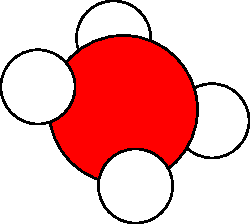
\includegraphics[width=0.2\linewidth]{bh4-flat}
\end{figure}

\section{Calcium Borohydride [$\beta$-\ce{Ca(BH4)2}]}
\label{sec:borohydrides-calcium}
The calculations were carried out using the Atomic Simulation Environment\footnote{\url{https://wiki.fysik.dtu.dk/ase/}}~\cite{ase-2002} and its implementation of the relevant algorithms.
The energies and forces were provided by the Dacapo plane wave DFT implementation~\cite{dacapo-1999}.
The calculational parameters can be found in DFT Calculations section of Paper \ref{pap:calcium}.
The calculational supercell was relaxed from the $P4_2/m$ space group ($\#84$)~\cite{cabh42-structure-p42m}, which contains two formula units, repeated once in each direction, totalling 176 atoms.

The bulk of the initial data from the QENS experiments indicated rotational diffusion of hydrogen, while possible high temperature long-range diffusion was also detected.
The experimental data suggested three unique processes, two of which were assigned to rotational diffusion of hydrogen, while the latter was assigned to longer range diffusion.
The work focused mainly on rotations around the possible symmetry axes, $C_2$ and $C_3$, of the \ce{BH4-} unit.

\subsubsection{Rotation of \ce{BH4-}}
By choosing appropriate axes, a contour plot of the rigid rotation was produced (\fref{fig:ca-pes01}) in order to get an overview of the possible rotations, pure or coupled, and an estimate of their relative barrier heights.

\begin{figure}[h]
\begin{center}
  \subfigure[Potential Energy Surface for \ce{Ca(BH4)2}][Potential Energy Surface for \ce{Ca(BH4)2} with MEPs and the local environment overlaid.]{
    \includegraphics[width=0.35\linewidth]{ca-pes01}
    \label{fig:ca-pes01}
    }
  \subfigure[\ce{Ca(BH4)2} energy profiles][\ce{Ca(BH4)2} energy profiles. The blue circles represent the $C_2$-type rotation and the red squares represent the $C_3$-type rotation.]{
    \includegraphics[width=0.45\linewidth]{ca-barriers}
    \label{fig:ca-barriers}
    }
    \parbox{0.85\linewidth}{
      \caption{The rotational analysis of \ce{BH4-} in \ce{Ca(BH4)2}.
      The figures are taken from paper \ref{pap:calcium}
It should be noted that some symmetry breaking can be seen in the PES, which is to be expected as the tetragonal symmetry is slightly broken during the minimisation, due to the environment.
      }
      \label{fig:ca-rotational}
    }
\end{center}
\end{figure}

Since the rotational system has three dimensions but the contour plot is limited to only two, the axes had to be chosen carefully as to sample all interesting events.
Each \ce{BH4} group has 3 nearest neighbour \ce{Ca} atoms and each $C_2$ axis roughly lines up with one of the three, nearly equivalent, \ce{Ca}-\ce{B} vectors, which means that with regards to symmetry they are also all nearly equivalent.
The one with maximal \ce{H}-\ce{Ca} distance was chosen as one of the contour axes.
The choice of the $C_3$ axis had a similar goal, to minimise \ce{H}-\ce{Ca} interaction.
This was accomplished by choosing the axis which lies closest to the plane spanned by the three nearest neighbour calcium atoms.
This axis samples half of the possible $C_3$ axes when the full $C_2$ rotation is taken into account.
Due to symmetrical similarity it is likely that the remaining $C_3$ axes are indirectly sampled also.

The contour plots give an important insight as to which of the possible rotations are the interesting ones and, thus, calculating the more resource intensive MEPs can be limited to the interesting processes.
\Fref{fig:ca-pes01} shows that a $C_3$ axis is lowest in energy and that a wobbly $C_2$ axis with a small intermediate minimum is the lowest energy $C_2$ type rotation.
Using these as the starting paths for NEB calculations, the MEPs, shown overlaid in \fref{fig:ca-pes01}, are found and shown as energy profiles in \fref{fig:ca-barriers}.

Right away, the theoretical data was in good agreement with the experimental data, nevertheless, further refinement of the experimental data was possible once the theoretical data for the rotations was complete, which yielded better agreement for the rotational data and an extra point for the possible long range diffusion.
This beautifully illustrates how theory and experiments complement and can be used to benefit each other.

In the end, the calculations complemented the experimental data very well, both with regards to the barrier height as well as the characteristic times which are derived from the HTST reaction rates (see Table 2 in Paper \ref{pap:calcium}).

\subsubsection{Long-range diffusion}
The remaining process was assigned to some sort of longer range hydrogen diffusion.
Multiple diffusional species and mechanisms can easily be imagined.
Vacancy mediated \ce{BH3},  \ce{BH4} and \ce{H} diffusion, interstitial hydrogen, atomic and molecular, and two different interstitial waters were all investigated with NEB calculations, and their results are shown in table 3 of paper \ref{pap:calcium}.

The vacancies all had high formation energies ($1.56\unit{eV}$ - $2.83\unit{eV}$) and barriers ($0.46\unit{eV}$ - $1.92\unit{eV}$) while the stable interstitial defects, had lower formation energies ($-0.05\unit{eV}$ - $0.40\unit{eV}$) and barriers ($0.09\unit{eV}$ - $0.68\unit{eV}$).
The \ce{H}-interstitial proved to be unstable and formed an \ce{H2}-interstitial coupled to an \ce{H}-vacancy.

The only defect that agreed to any significance with the experimental data, was the \ce{H2}-interstitial, with a barrier of $0.09\unit{eV}$ (exp. $\mytilde0.12\unit{eV}$) and diffusional length of $2.1\unit{\mAA}$ (exp. $\mytilde2.5\unit{\mAA}$).
The characteristic times were, however, not in agreement (theoretical $0.06\unit{ps}$ vs. exp. $4\unit{ps}$).
These discrepancies might very well be due to the lack of experimental data points, since only two were available for a linear interpolation on an Arrhenius type plot (figure 10 in paper \ref{pap:calcium}).

\section{Magnesium Borohydride [$\beta-$\ce{Mg(BH4)2}]}
\label{sec:borohydrides-magnesium}

%\bit
%\item Calculate rigid rotations of \ce{BH4-} to get a "feel" for the landscape for all the different borons in the cell
%\item Show multiple PESes
%\item Then calculate the reaction paths (MEPs) and saddle points
%\item Prepare HTST rates and compare with experiments
%\item Flat landscape $\rightarrow$ Introduce the next section
%\eit

The calculational supercell was relaxed, from the $fddd$ spacegroup ($\#70$), totalling 176 atoms.
The structure consists of 5 symmetry inequivelant \ce{BH4} sites which all have similar local structure, being wedged between 2 \ce{Mg} atoms (\fref{fig:mg-local-structure}).
The symmetry inequivilance stems from the fact that each \ce{BH4} was slightly away from the \ce{Mg}-\ce{Mg} axis.
The distance, $L$, from the \ce{B} to the axis, influences the barriers.

\figmiss{Environment, for explaining the axes used}

The experimental data detected only rotational diffusion.
Thus, the work exclusively revolved around understanding which rotations correpsonded with the experiments.

For each inequivelant site a number of rigid rotation PESes were constructed in order to get an overview of the interesting events and to limit computations spent on the MEP calculations, similar to \fref{sec:calcium}.
Due to symmetry not all the axes needed to be considered.

The general result from the PESes was that rotations that maximised the \ce{Mg}-\ce{H}, $d_{H-Mg}$ distance showed the lowest energies (\fref{fig:h-mg-distances}).
In this respect, two distinct types of $C_2$ axes were seen, those parallel to the \ce{Mg}-\ce{Mg} axis, $C_2^\parallel$, which maximised $d_{H-Mg}$ and those perpendicular to it, $C_2^\perp$, where $d_{H-Mg}$ was generally lower and had higher barriers.
MEP calculations for the latter found a combination of other axes yielded the same permutation but at a much lower energy cost.
The difference in relative barrier height decreased with decreasing $L$.\footnote{The relative difference would be non-existant for $L=0$ but non of the \ce{BH4} fulfill that critrion.}

\begin{figure}[h]
\begin{center}
  \subfigure[Average \ce{H}-\ce{Mg} distance]{
    \includegraphics[width=0.45\linewidth]{h-mg-distances-avg}
    \label{fig:h-mg-distances-avg}
    }
  \subfigure[Minimum \ce{H}-\ce{Mg} distance]{
    \includegraphics[width=0.45\linewidth]{h-mg-distances-min}
    \label{fig:h-mg-distances-min}
    }
    \parbox{0.85\linewidth}{
      \caption{\ce{H}-\ce{Mg} distances of the points that constitute all the PESes that were produced.
Some systemaitc features can be seen since the data was produced with specific rotations rather than a uniform distirubtion.
A clear trend for lower energies with higher distances can be seen.
      }
      \label{fig:h-mg-distances}
    }
\end{center}
\end{figure}

\figmiss{The different gengeral types of PESes.}

No such clear distinction could be made with regards to the $C_3$ axes.
However, due to symmetry all the $C_3$ axes for a given site yield a very similar PES. \tblue{(Should I show the four PESes for B04?)}

The rigid rotation plots are not able to give a full description of the events, neither their geometry nor their energetics.
Thus MEP calculations were performed with the lowest energy rigid rotation paths as starting guides.
The barriers from 

\figmiss{Barrier dependancy on distance}

It is unsurprising to find that there is a direct relationship between $L$ and the $C_2$ barrier height.
In fact, the relationship is linear, as can be seen in \fref{fig:mg-barriers}, with increased $L$ the barrier increases which is most likely due more \ce{H}-\ce{Mg} interaction.
On the other hand, no such direct relationship could be found for the $C_3$ axes.

\incomplete

\section{Summary}
\label{sec:borohydrides-summary}

Collaboration between experimental work and theoretical work was able to produce a convincing image of the low temperature rotational motion of two borohydrides --- both of which have very high hydrogen capacity ---, a task hindered by the scarcity of appropriate experiments.

When considering a system of events of such a different nature, rotational diffusion on the one end and long range diffusion on the other, lead to thoughts on what actually lies between the similar events, in this case the rotational diffusion events.
The PESes give some indication as to what sort of \sap{2} seaparates the events but as with the MEPs, the rigid rotation barriers are insufficient.
Thus was born the idea to find the \sap{2} exactly, using a NEB type method, and this effort will be discussed in detail in \fref{chap:erm} and Paper \ref{pap:second-order}.

\incomplete


\chapter{Beyond Harmonicity \pending}
\label{chap:erm}

In this chapter, the methodology part of paper \ref{pap:second-order} is first summarised and then expanded on.

\section{Introduction}
\label{sec:erm-introduction}
% -----------------------------------------------------------------

A collection of two specific steepest descent paths starting infinitesimally close to a \sap{2} and ending at the neighbouring \sap{1}s can be considered a ridge.
Such a path is non-trivial to find as information about the curvature, the Hessian, is essential but often unavailable in a direct manner.

A given point, $\vR$, is located on a ridge if its gradient is parallel with its tangent and the Hessian matrix for a reduced space where the tangent is excluded has a single negative eigenvalue~\footnote{Higher order "ridges" can be identified if the Hessian has more negative eigenvalues.}.

A method for iteratively aligning a path with the ridge is presented, building on the well established NEB (\fref{sec:neb}) and Dimer \fref{sec:dimer} methods.
This method is then applied to the self diffusion of an adatom on the \ce{Al}(100) surface in \fref{chap:al}.

After converging to the ridge, the validity of the harmonic approximation to transition state theory (HTST) is considered and an improvement to the reaction rate offered.


\section{Ridge Mapping}
\label{sec:ridge-mapping}
Given a function, $E$, of multiple variables, $\vR$, its gradient, $\nabla E(\vR)$, and two \sap{1}s, the goal is to identify a path that lies close to the ridge between the \sap{1}s.
The path should, in particular, lie through any intermediate \sap{2}s so that a comparison of their height with respect to the endpoints can be made.
The method should, furthermore, lead to the identification of previously unknown \sap{1}(s) on the ridge in between the given end points, should they exist.

\subsubsection{Gradient Modification}
\begin{SCfigure}[5.0][h]
\centering
\includegraphics[width = 0.35\linewidth]{erm-forces}
\caption{
The construction of the effective force, $\vF^\text{eff}_i$,
which acts on image $i$ of the path and is used in the iterative optimisation.
The solid grey line indicates the ridge,
the black filled circles represent the current location of three adjacent images,
the black solid line shows the tangent estimate, $\uvt_i$
and the black dashed line shows the minimum mode estimate, $\uvn_i$.
The orange arrow shows the gradient force, $\vF_i= -\nabla E$.
The red arrow shows the transformed force, $\vF^t$ (\fref{eq:transformed-force}).
The purple arrow shows $\vF_i^\perp$, the transformed force(\fref{eq:transformed-force}),
The green arrow shows $\vF_i^\text{S}$ (\fref{eq:full-spring-force}),
The blue arrow shows $\vF_i^\text{eff}$ (\fref{eq:erm-effective-force}).
Due to the limited dimensionality of the figure, $\vF_i^\perp$ and $\vF_i^\text{t}$ appear to be parallel to $\uvn_i$, but this is generally not the case for real systems.
}
\label{fig:erm-forces}
\end{SCfigure}

Similarly to the NEB method~\cite{neb-original-1998} (\fref{sec:neb}), a path of $N$ discrete images, $[\vR_0, \vR_1, \ldots, \vR_N]$, is iteratively aligned with the ridge by modifying the gradient or force, $\vF_i \equiv -\nabla E(\vR_i)$, for each one.
However, unlike the NEB method, further force modifications are needed, in order to converge to a ridge rather than a MEP.

The path is at each image defined by its tangent, $\uvt_i$, and in order for the path to be at a SDP (such as the ridge), any force components perpendicular to it,
\beq{perpendicular-force}
\vF_i^\perp \equiv \vF_i -(\vF_i \cdot \uvt_i)\uvt_i,
\eeq
must be zero,
\beq{ridge-force}
\vF^\perp_\text{ridge} = \vect{0}.
\eeq
Furthermore, one negative eigenvalue of the Hessian, perpendicular to the path, must be guaranteed.\footnote{If finding higher order ridges is desired, more negative eigenvalues must be guaranteed.}
The Dimer methodology~\cite{dimer-original-1999, dimer-olsen-2004} (\fref{sec:dimer}) for finding the lowest eigenvalue and the corresponding eigenvector (minimum mode) of the Hessian, $\uvn_i$, can produce a transformed force,
\beq{transformed-force}
\vF_i^\text{t} = \vF_i^\perp - 2(\vF_i^\perp \cdot \uvn_i)\uvn_i,
\eeq
that will map concave degrees of freedom to convex ones, effectively making the ridge appear as a MEP with regards to the gradient.
Since eigenvectors are not necessarily perpendicular to the ridge (as can be seen in figure 1 of paper \ref{pap:second-order}), the path itself must be left out of the Hessian's vector space, thus applying an orthogonality constraint on the minimum mode,
\beq{orthogonality-constraint}
\uvt_i \cdot \uvn_i = 0,
\eeq
at all times.

Similarly to the NEB method, an artificial force is employed in order to keep the images equally\footnote{or with controlled spacing} distributed along the path.
For the NEB method this force acts only along the path and is generally referred to as the spring force as it resembles springs connecting the images,
%However, in the case of ridge calculations, the full spring force must be used,
\beq{full-spring-force}
\vF_i^\text{S} = k \left[ \left( \vR_{i+1} - \vR_i \right) - \left( \vR_i - \vR_{i-1} \right) \right],
\eeq
where $k$ is the spring constant, which controls the stiffness of the springs.
In the NEB, only the component along the path must be included, however, for ridge calculations retention of the full spring force is necessary due to numerical instabilities which proved to be more prominent in ridge calculations than MEP calculations (see below).

Combining the above forces, $\vF_i^\text{t}$ and $\vF_i^\text{S}$, into an effective force (as shown in \fref{fig:erm-forces}),
\beq{erm-effective-force}
\vF_i^\text{eff} = \vF_i^\text{t} + \vF_i^\text{S},
\eeq
will allow the path to converge close to the ridge.

\subsubsection{Exact Convergence to the \sap{2}}
Beyond the problems already discussed regarding converging exactly to the \sap{1} in NEB calculations, systematic errors due to the retention of the full spring force makes it unlikely that using only \fref{eq:erm-effective-force} will yield an image at the exact \sap{2}.
As with the NEB method a Dimer-type solution is possible --- similar to equations \ref{eq:dimer-transform} and \ref{eq:neb-ci-transform} --- where the highest value image is decoupled from the springs, forming the so-called climbing image, and force components along the \emph{two} lowest eigenvalued eigenmodes, as defined by the minimum mode and the tangent,
\beq{erm-ci}
\vF_{i_\text{max}}^\text{eff} = \vF_{i_\text{max}} - 2(\vF_{i_\text{max}} \cdot \uvt_{i_\text{max}})\uvt_{i_\text{max}} - 2(\vF_{i_\text{max}} \cdot \uvn_{i_\text{max}})\uvn_{i_\text{max}},
\eeq
where $i_\text{max}$ refers to the image with the highest functional value.

The introduction of the climbing image ensures convergence to the highest \sap{2} along the ridge, analogous to the convergence to the \sap{1} in an NEB calculation.
However, in the ridge calculation it additionally reduces the corner cutting of the path in the neighbourhood of the \sap{2}.
The added computational effort involved with the climbing image calculation is, therefore, not easy to measure in the case of the ridge calculation since it affects the extent to which the path converges to the ridge.
Furthermore, this addition can not be considered optional, as it can technically for NEB, since it serves as an indirect stabilisation tool at the top of the path, where the environment is concave in 2 dimensions rather than 1 as is the case with a MEP.

%Unlike the NEB, the computational effort involved in introducing the climbing image is not easily measured due to the systematic errors introduced by the full spring force\footnote{NEB calculations and NEB-CI calculations converge to the same path with different image placements, while ridge calculations suffering from corner cutting near the \sap{2} and those who do not, converge to different paths.} but there is no reason to suspect increased effort by applying \fref{eq:erm-ci}.

\subsection{Numerical Instabilities}

\subsubsection{The Orthogonality Constraint}
\begin{figure}[htb!]
\begin{center}
  \subfigure[The higher-image tangent is used for the orthogonality constraint of the minimum mode.]{
    \includegraphics[width=0.45\linewidth]{orthogonal-bad}
    \label{fig:orthogonal-bad}
    }
  \subfigure[A central difference tangent is used for the orthogonality constraint of the minimum mode.]{
    \includegraphics[width=0.45\linewidth]{orthogonal-good}
    \label{fig:orthogonal-good}
    }
    \parbox{0.85\linewidth}{
\caption{
The ridge is the black dashed line.
The white arrows are the PES force, the grey arrows are the dimer transformed forces and the black arrows are the effective forces.
The red line is the higher-image tangent and the blue line is the minimum mode estimate.
The system is a frozen 1 layer \ce{Al}(100) "slab" with a free to move \ce{Al} adatom, modelled with EMT~\cite{emt-1996} and the ridge is that between two neighbouring hop \sap{1}s.
The PES is created by relaxing the adatom in the direction perpendicular to the frozen layer.
Shown are the in-plane components of the forces and vectors.
The out-of-plane components for all are very small.
}
\label{fig:orthogonal}
}
\end{center}
\end{figure}

Simply using the Dimer, or any other non-exact, estimate of the minimum mode introduces instabilities in the forces, as the ridge$\rightarrow$MEP mapping can get inaccurate.
This is not a problem hindering convergence, directly, since the Dimer generally has ample time to converge to the nearly exact minimum mode during the iterative convergence.

More serious seems to be the interaction between the minimum mode and the tangent, as enforced by \fref{eq:orthogonality-constraint}.
The tangent is designed to minimise numerical instabilities in the NEB~\cite{neb-tangent-2000} but not to offer a particularly good estimate of the path's tangent at any given time, however, once converged, it offers a reasonably good estimate\footnote{A better estimate of the steepest descent path in question (the minimum energy path) would be a tangent pointing downwards rather than upwards.} and in the limit of infinite amount of images, an exact tangent.
Using a tangent that depends on both neighbouring images, the path would form kinks under minute perturbations that would not even out with more iterations.
The orthogonality constraint (\fref{eq:orthogonality-constraint}) propagates a similar error in the minimum mode estimate under perturbations to the path.
This, in turn, introduces similar instabilities as the kinks, when the ridge$\rightarrow$MEP mapping becomes inaccurate (\fref{fig:orthogonal-bad}).
Preliminary testing showed that this is not a problem where individual degrees of freedom were decoupled (non-interacting) but for systems where all degrees of freedom interact (most systems) such instabilities are problematic and common.

In paper \ref{pap:second-order}, these instabilities are reduced by the inclusion of the perpendicular spring force component which yields the more systematic error of corner cutting (discussed below).
Further analysis showed that enforcing the orthogonality constraint (\fref{eq:orthogonality-constraint}) using a tangent estimate that is focused on accuracy, rather than stability, reduces the problematic behaviour (\fref{fig:orthogonal-good}).
The system would then have two tangent definitions co-existing, a numerically stable one for the NEB-type force scheme (\fref{eq:perpendicular-force}) and a more accurate representation of the ridge,
\beq{central-difference-tangent}
\uvt_i^\text{ridge} = \frac{\vR_{i+1} - \vR_{i-1}}{\left| \vR_{i+1} - \vR_{i-1} \right|},
\eeq
for the projection of the Hessian (\fref{eq:orthogonality-constraint}).
This latter scheme was neither employed in paper \ref{pap:second-order} nor \fref{chap:al} and has not been tested fully.
Nevertheless, the initial results are promising for the removal/reduction of corner cutting.

\Fref{fig:orthogonal} demonstrates the problem and suggested solution.
However, the problem seems to be system specific and dependant on, at least, the curvature of the contour lines.
In order to fully understand the root cause of these instabilities, more research on more test systems is required but using the tangent from \fref{eq:central-difference-tangent} seems to be a vital step.
In fact, the test cases considered would generally converge to the exact ridge without the use of the perpendicular spring force if started from a path that had been converged with the full spring force.
This was not the case for all systems test but those with only mild corner cutting would all converge.

\subsubsection{Non-barrier profiles}
\begin{SCfigure}[10][htb!]
\centering
    \includegraphics[width=0.45\linewidth]{bad-energy-profiles}
\caption{A schematic of some of the possible initial energy profiles of a ridge calculation.
A barrier (black, solid), a monotonic decrease (blue, dotted) and an inverted barrier (red, dashed).
Only the first is possible in NEB calculations.
}
\label{fig:bad-energy-profiles}
\end{SCfigure}

Since the end points of the ridge are not local minima, there is no intrinsic barrier separating them, as is the case for NEB calculations.
In fact, the initial profile can have any shape, including a monotonic one or even an inverted barrier, if it lies near a local minimum, which is \emph{not} unlikely, examples of which can be seen in \fref{fig:bad-energy-profiles}.
This means that the initial environment of the path is drastically different from that of the ridge.
To help bring the path nearer to the ridge, the full spring force was used.
Furthermore, the usage of the climbing image becomes questionable as the immobile end images may very well be the highest ones.
If using the climbing image from the outset is required, non-highest images must be used as the climbing image.
Images numbered $1$ and $N-1$ are partially restrained by the immobility of the endpoints, thus images even further in must be used, $2$ or $N-2$.

\section{Corner Cutting}
\label{sec:erm-corner-cutting}

Should finding the exact ridge be the goal --- rather than just the \sap{2} and a ridge estimate --- and the alternative tangent discussed above not be sufficient, multiple strategies can be envisioned, all of which aim at somehow reducing the perpendicular component of the spring force while avoiding or minimising the instabilities discussed above.

\subsubsection{What is corner cutting}
The spring force tries to keep each image as close as possible to its neighbours.
Without any further influence, the images would align evenly spaced in a straight line.
However, since there are other forces at work, perpendicular to the path, $\vF^\text{t}$, an equilibrium between the conflicting forces will be reached, when they are equal in length but with opposite direction,
\beq{corner-cutting-equilibrium}
\vF^{\text{S}\perp} = -\vF^\text{t},
\eeq
producing a systematic error which is commonly referred to as corner cutting.
Since the goal of the whole method is to fulfil \fref{eq:ridge-force}, such an equilibrium can be unsatisfactory.

This problem existed in the infancy of NEB calculations but was made a thing of the past with more numerically suitable tangent and spring force definitions.~\cite{neb-tangent-2000}
These changes are not directly applicable to ridge calculations due to intrinsic stability issues which are dampened by the perpendicular component of the spring force.
However, once the path is sufficiently well behaving and near the ridge, minimising the corner cutting could be done.

\figmiss{Graphic representation of corner cutting. Medium priority.}

\subsection{Minimise corner cutting}
\textit{After publishing paper \ref{pap:second-order} some effort went into finding the exact ridge instead of paths that suffer from corner cutting.
The methods and ideas presented here serve more as a detailed outlook for future work than a complete study.}
\vspace{1em}

In order to reduce/remove corner cutting, the perpendicular component of the spring force must be removed/reduced at each image.
Then in tune with the equilibrium presented in \fref{eq:corner-cutting-equilibrium}, \fref{eq:ridge-force} will be fulfilled and the exact ridge found.

Using the dual tangent scheme, presented above, it is possible to significantly reduce the numerical instabilities of the ridge calculation.
In some test cases even allowing for the complete exclusion of the perpendicular spring force after turning on the climbing image.
However, should this not be possible, a multiplication factor, $\xi_i \in [0, 1]$, for the perpendicular spring force,
\beq{spring-force-perpendicular}
\vF_i^{\text{S}\perp} = \vF_i^\text{S} - (\vF_i^\text{S} \cdot \uvt_i)\uvt_i,
\eeq
can be defined,
\beq{spring-force-reduction}
\vF_i^{\text{S, eff.}\perp} = \xi_i \vF_i^{\text{S}, \perp},
\eeq
to iteratively bring the effective perpendicular component, $\vF_i^{\text{S, eff.}\perp}$, to zero and thus converging to the exact ridge.

Multiple schemes for reducing $\xi_i$ can be envisioned.
One, that initial testing showed to be successful, is reducing $\xi_i$ each time corner cutting is detected and then continuing the iterative convergence until either corner cutting is detected again or the path is fully converged to the ridge.
By how muchi $\xi_i$ is reduced each time, could either be a fixed ratio or, preferably, dependant on the amount of corner cutting.\footnote{Only the fixed ratio scheme was tested.}
In order for the path to converge evenly, $\xi_i$ must be constricted to be within a certain range of $\xi_{i-1}$ and $\xi_{i+1}$.
Using a scheme such as this, the corner cutting was significantly reduced in the test systems\footnote{Both custom potentials and the Al self diffusion (\fref{chap:al}) systems were tested but not extensively.} it was applied to.

It warrants repeating that the ridge method, as presented originally in paper \ref{pap:second-order}, is able to find the \sap{2} exactly without problem but if the ridge is curved, corner cutting will take place.
While the removal of corner cutting would present a truer picture of the ridge, the method as it stood is still of good use.

%The main problem with simply removing the perpendicular spring force is the instabilities that exist due to the orthogonality constraint (see above) of \fref{eq:orthogonality-constraint}, which in turn is employed to overcome other instabilities.

\begin{comment}
\subsection{Older stuff}

\bit
\item Iteratively remove parts of $\vF^\text{S}_\perp$ and relax
\item Detect corner cutting ($\hat{\vF^\text{t}_\perp} \cdot \hat{\vF^\text{S}}_\perp \approx -1$ and $|\vF^\text{t}_\perp| \approx |\vF^\text{S}_\perp|$). Maybe detect a cone around the corner cutting direction and reduce containment there for the next steps also.
\eit
I've tried both with moderate to good success rate on the hop diffusion of Al (EMT).
Need to move on to more complicated systems (concerted self-diffusion of Al).

--- Minor fluctuations in the tangent ... 

A possible "solution" is to keep the dimer fixed after switching to the "reduce corner-cutting phase" but then the dimer WILL be wrong after a few iteration in the last phase.
Maybe the answer is to take an average of previous tangents, etc.

Since there is no guarantee that the eigenmodes align with the tangent and minimum mode at all points on the ridge (see \fref{fig:modes}), it is not advisable to let go of the orthogonality constraint between the minimum mode and the tangent,
\beq{orthogonality-constraint}
\uvn \cdot \uvt = 0.
\eeq
Early tests of releasing the constraint on some of the images were not reliable.

\incomplete

\subsubsection{\tblue{Informal Babble}}

I have two ideas that I'm currently working on.
\paragraph{The first scheme}
By gradually removing $\vF^{\text{S}\perp}$, the path is brought closer to the true path.
There are multiple ways to do this but the way I do it currently is to detect the corner cutting and its direction.
When the perpendicular spring force and the perpendicular transformed force are pointing in opposite directions,
\beq{asdf1}
\frac{\vF^{\text{t}\perp}_i}{|\vF^{\text{t}\perp}_i|} \approx -\frac{\vF^{\text{S}\perp}_i}{|\vF^{\text{S}\perp}_i|},
\eeq
and their length is the same,
\beq{asdf2}
|\vF^{\text{t}\perp}_i| \approx |\vF^{\text{S}\perp}_i|,
\eeq
corner cutting has taken place.
When these criteria are satisfied, $\vF^{\text{S}\perp}_i$ is permanently decreased by a factor, $\xi_i$,
\beq{asdf3}
\vF^{\text{S}\perp\text{eff}}_i = \vF^{\text{S}\perp\text{full}}_i \xi_i.
\eeq
Currently there is no good way to decide how much $\xi_i$ is decreased when corner cutting is detected but it should be easy to devise a scheme.

This has worked well on the hop-hop test system in multiple dimensions to reduce the corner cutting significantly (90\%) but not fully as the band becomes unstable (in particular when many images are used, above 40).

\paragraph{The second scheme}
It seems that there are two conflicting factors that hinder finding the true path.
\bit
\item When the tangent and dimer are kept perpendicular to each other, kinks seem to form in the band (I have not managed to fully understand why) and once this happens, everything goes bad quickly
\item This  seems to be less of a problem when the dimer is allowed to freely rotate but allowing this in systems where the true eigenmodes do not align with the ridge yields forces that quickly pull the band far off the ridge. 
\eit

Initial testing (on the hop-hop system) shows that changing the eigenmode-tangent orthogonality constraint to use a different tangent ($\vR_{i+1} - \vR_{i-1}$) which is more similar to the real ridge when an image gets slightly off the ridge, yields up to $100\%$ reduction of corner cutting, when used along with a complete removal of $\vF^{\text{S}\perp}$.

The current tangent (which only depends on the displacement to the top energy image) is less accurate but works better due to stability issues (kinks do not form).

It does seem that alining the dimer perpendicular to the ridge is essential because otherwise the significantly sized force that lies along the ridge (and should get "nudged" out) get deflected and produces a force in the wrong direction.

\paragraph{Scheme 1.5}
How about applying the first schem from the Saddle point downwards.
Either converging points $i_\text{max} \pm 1$ and then locking them in place (similar to the CI) and then converging points $i_\text{max} \pm 2$, etc.

OR using the first cheme but never allowing constricting $\xi_i$ to be higher than for the neighboring higher energy image.

It is very easy to try this latter implementation but the first one requires a bit of programming.

\paragraph{Measuring corner cutting}
The corner cutting is measured by dotting together the effective force and the tangent,
\beq{asdf4}
\text{measure} = \frac{\vF_i^\text{eff}}{|\vF_i^\text{eff}|} \cdot \uvt,
\eeq
When this is $1$, there is no corner cutting.

\end{comment}

\section{Testing}
\label{sec:erm-testing}
% ------------------------------------------------------------------

\placeholder



\chapter{Self diffusion of aluminium}
\label{chap:al}
\section{Introduction}
\label{sec:al-introduction}

\bit
%\item The Dimer has been used succesfully on the system
%&\item The system is easy to calculate (EAM)
\item Good real world example to test the ridge method on (Both similar and dis-similar events present) at a reasonable computational cost.
\item Corner-Cutting?
\eit

This system was chosen as a test case for the ridge method \expand
The dimer method, on which the current implementation of ridge calculations heavily depends, has been used succesfully on the system~\cite{dimer-original1999}, using the well tuned and fast embedded atom method (\fref{sec:potentials})~\cite{eam-1983, eam-1986}.

\incomplete

\section{Energy Ridges}
\label{al-energy-ridges}

The energy ridges between all the lowest energy \sap{1}s were calculated.
Two situations of particular interest arose.
The first was the discovery of intermediate \sap{1}s, while the second concerned the HTST reaction rate, its accuracy and efforts to improve it.

\subsubsection{Intermediate \sap{1}s}
\begin{figure}[hp]
\begin{center}
\includegraphics[width = 1.0\linewidth]{discovery}
\caption{
Calculated path at the ridge between the \sap{1}s for a hop and concerted 4-atom displacement.
The circles show the position of converged images (coloured circles for \sap{1}s and \sap{2}s, but grey for the rest). 
These \sap{1}s turned out not to be adjacent on a ridge and the path optimisation reveals an intermediate \sap{1}, the one for the concerted 2-atom displacement.
%This illustrates how a ridge calculation could reveal new and possibly unknown transition mechanisms.
The long path is not able to accurately locate the intermediate \sap{1} and the lower energy \sap{2} due to finite resolution in the discretisation and corner-cutting.
The exact configuration of the \sap{1} can be found using a \sap{1} finding algorithm starting with the approximation obtained from the optimised path.
Then, a calculation of a shorter path, between the \sap{1}s of the 2-atom  and 4-atom displacements, locates the intermediate \sap{2} accurately (cyan circle)
The insets show an overlay of three configurations, two adjacent \sap{1}s and the intermediate \sap{2}.
The atom colours correspond to the coloured spheres of the energy ridge.
}
\label{fig:discovery}
\end{center}
\end{figure}

As can be seen in \fref{fig:discovery} there is a significant energy ridge "barrier" separating the hop and concerted 2 atom \sap{1}s.
More interestingly, ridge calculations between the more populous concerted \sap{1}s (3 and 4 atom) and the hop revealed that they were interspersed with the concerted 2 atom \sap{1}.
This is not surprising as the concerted mechanisms are all quite similar with regards to their coordinates, while the hop mechanism is inherently different.

Finding the intermediate \sap{1} is only accurate in the limit of an infinite amount of images and no corner cutting, but the lowest energy image gives a good starting guess, both for the coordinates and the minimum mode, for traditional \sap{1} methods, such as the Dimer.
It would be possible to implement a "sinking" image alteration of the effective force in a manner similar to the climbing image but this was not done here.
Similarly, corner cutting prevents rigorous convergence to the lower energy \sap{2}.
A second climbing image would converge exactly to this point but this was not done.\footnote{Implementing multiple climbing or sinking images is in principle not difficult but the ramifications could be dire, e.g. in systems with rugged landscapes and a limited amount of images.}
However, performing a second ridge calculation with the intermediate \sap{1}(s) as end points yields the exact \sap{1} and, apart from the possible corner cutting, the ridge.
These latter paths are displayed as red curves in \fref{fig:discovery}

\subsubsection{Beyond Harmonicity}
\begin{figure}[hp]
\begin{center}
\includegraphics[width = 1.0\linewidth]{low-barriers}
\caption{
The energy ridge going through \sap{1}s of 2-atom, 3-atom, 4-atom and, then the same, 2-atom concerted displacement for an Al adatom on a Al(100) surface.
The circles represent the position of images in the optimised paths, the \sap{1}s and the \sap{2}s being coloured differently but the rest coloured grey.
The green curves represent harmonic approximations to the energy surface at each \sap{1}.
The insets show an overlay of three configurations, two adjacent \sap{1}s and the intermediate \sap{2}.
The atom colours correspond to the coloured spheres of the energy ridge.
}
\label{fig:low-barriers}
\end{center}
\end{figure}

\begin{figure}[hb]
\begin{center}
\includegraphics[width = 0.5\linewidth]{integral-ratios}
\caption{
The harmonic correction ratio, $\Gamma$, defined in \fref{eq:htst-correction-factor},
between the configuration integrals of the potential energy ridge shown in \fref{fig:low-barriers} and the corresponding harmonic approximations.
The lines represent the ratio for individual processes: concerted 2 atom (blue, dotted), 3 atom (green, dashed), 4 atom (red, dash-dotted) and the ratio for all the processes combined (black, solid).
%The black, solid, line is the ratio for the full integral, including all three concerted displacement processes.
%The blue, dotted, line is the ratio when only considering the 2-atom concerted displacement.
%The green, dashed, line is the ratio when only considering the 3-atom concerted displacement.
%The red, dash-dotted, line is the ratio when only considering the 4-atom concerted displacement.
For the individual processes, the end points of the ridge integral are the adjacent \sap{2}s, while the full integral is done for the whole ridge.
%While the harmonic approximation gives a good approximation for the total configuration integral over the whole temperature range shown, because it is dominated by the 2-atom displacement, the estimate for each of the 3-atom and 4-atom displacements is poor unless the temperature is very low.
}
\label{fig:integral-ratios}
\end{center}
\end{figure}

The ridges between the, similar, concerted motion \sap{1}s are shown in \fref{fig:low-barriers}.
It can be clearly seen applying HTST to the concerted 3 and 4 atom \sap{1}s is highly questionable as their neighbouring \sap{2}s are very low, $\mytilde 0.005\unit{eV}$ and $0.012\unit{eV}$, certainly lower than the $5\kB T$ rule of thumb\footnote{at any temperature above $9\unit{K}$ and $28\unit{K}$ respectively.}.
However, applying HTST to the concerted 2 atom mechanism is more justified, by visual inspection the ridge is fairly near harmonicity up to the $5\kB T = 0.128\unit{eV}$ limit at room temperature and the \sap{2}s are still higher.
\Fref{fig:integral-ratios} further shows that the concerted 2 atom rate has a correction factor, $\Gamma$, of approximately $1.0$ throughout the temperature range while the concerted 3 and 4 atom mechanisms have significant correction factors at all temperatures.

It might appear wise to rigorously calculate such a correction factor for all the degrees of freedom until one considers the complexity of such an exercise.
Figure 6 in paper \ref{pap:second-order} makes an effort to put into context the abundance of ridges on which each \sap{1} lies but, of course, fails to do so properly due to the immense dimensionality (771 degrees of freedom) of the PES.
Not only finding all the \sap{1}s leading out of a given basin but also finding all neighbouring \sap{2}s and ridges for each one would be folly due to the sheer amount of possible \sap{}s.
Furthermore, as stated when introducing the correction factor, $\Gamma$ is not a rigorous correction factor and should not be used as such.
However, using the ridge to calculate a more precise reaction rate, outside the HTST framework, seems appropriate and will make an interesting subject for future research.

\subsubsection{Performance}
Theoretically, ridge calculations should scale like the NEB effort times the Dimer effort, i.c. 3 times the NEB effort.
However, directly comparing the determination of MEPs to the determination of ridges is unfair, \expand



\chapter{Coupled Hydrogen Defects in Perovskites}
\label{chap:perovskites}

\textit{This chapter briefly describes testing the ridge method for a complex DFT system.}

\section{Introduction}
\label{sec:perovskites-introduction}

This chapter describes work performed to further understand the coupled hydrogen defects in perovskites.
The original work was based on ... cite


% ------------------------------------------------------------------
\placeholder



\chapter{Summary}
\label{chap:summary}

The rotational dynamics of two complex borohydrides were investigated in detail with close collaboration to experimental work.

A method for detecting energy ridges (easily applicable to any multidimensional function) was developed.
By combining the dimer algorithm for mapping convex regions to concave regions, i.c. first order saddle points to minima and ridges to minimum energy paths, and the nudged elastic band algorithm for finding minimum energy paths


\bit
\item Mapping ridge paths is achieved using a novel way of combining previously well established \sap{1} algorithms.
\item \expand
\item Initial attempts at DFT ridges were promising when the initial guesses were good enough but minima trapping was an unexplained problem
\eit

\placeholder






\section{Outlook}
\label{sec:summary-outlook}

A detailed outlook as to further development of the ridge detection algorithm was presented in \fref{chap:erm}.


Finding further use for the energy ridges will be interesting.
For example, stitching together a transition state from hyperplanar segents near each image of every ridge (with the minimum modes as normals), where the amount of images could possibly viewed as a variational parameter in lieu of the transition state.


\bit
\item DFT ridges
\item How ridge calculations interact with different types of saddle points (such as those with $H = \vect{0}$, SPs which are also points of inflection or turning points)
\item Rigorous performance study.
\item Discover the limit of how low \sap{2} can be with regards to \sap{1}. i.e. confirm the $5\kB T$ stuff.
\item Use ridges to create full transition states with the dimer as normal to a hyperplanar segment
\item Catalytic Selectivity
\item Extend to Quantum HTST
\eit

\placeholder



% Create the bibliography
\newpage
\addcontentsline{toc}{chapter}{Bibliography}
\bibliography{thesis}

% Using pdfpages strips all links from the pdfs. There is a package called pax that restores some (all?) of the links. Check it out if you have the time.
\part{Papers}
\label{part:papers}
\appendix
% Hack the "Chapter" names
%\newcommand{\appchapter}[1]{\let\oldthechapter\thechapter
%  \renewcommand{\thechapter}{Paper \oldthechapter}
%    \chapter{#1}\let\thechapter\oldthechapter}

%\appchapter{Hydrogen Rotational and Translational Diffusion in Calcium Borohydride from Quasielastic Neutron Scattering and DFT Calculations}
%\label{pap:calcium}
\includepdf[pages=1, addtotoc={1,chapter,0,Hydrogen Rotational and Translational Diffusion in Calcium Borohydride from Quasielastic Neutron Scattering and DFT Calculations,pap:calcium}]{papers/calcium.pdf}
%\includepdf[pages=-, openright, fitpaper, addtotoc={1,chapter,0,Hydrogen Rotational and Translational Diffusion in Calcium Borohydride from Quasielastic Neutron Scattering and DFT Calculations,pap:calcium}]{papers/calcium.pdf}

%\appchapter{Hindered Rotational Energy Barriers of \ce{BH4-} Tetrahedra in $\beta$-\ce{Mg(BH4)2} from Quasielastic Neutron Scattering and DFT Calculations}
%\label{pap:magnesium}
\includepdf[pages=1, addtotoc={1,chapter,0,Hindered Rotational Energy Barriers of \ce{BH4-} Tetrahedra in $\beta$-\ce{Mg(BH4)2} from Quasielastic Neutron Scattering and DFT Calculations,pap:magnesium}]{papers/magnesium.pdf}
%\includepdf[pages=-, openright, fitpaper, addtotoc={1,chapter,0,Hindered Rotational Energy Barriers of \ce{BH4-} Tetrahedra in $\beta$-\ce{Mg(BH4)2} from Quasielastic Neutron Scattering and DFT Calculations,pap:magnesium}]{papers/magnesium.pdf}

%\appchapter{A method for finding the ridge between saddle points applied to rare event rate estimates}
%\label{pap:second-order}
\includepdf[pages=1, addtotoc={1,chapter,0,A method for finding the ridge between saddle points applied to rare event rate estimates,pap:second-order}]{papers/second-order.pdf}
%\includepdf[pages=-, openright, fitpaper, addtotoc={1,chapter,0,A method for finding the ridge between saddle points applied to rare event rate estimates,pap:second-order}]{papers/second-order.pdf}

\end{document}
